\section{El Mundo y la Máquina}

Los primeros conceptos que detallaremos estarán involucrados con la ingeniería de los requerimientos. Los puntos de vista
más relevantes son los de Zave y Jackson (\cite{Zave97fourdark, Jackson:1995:SRA:210207, 5071113}) por un lado, y los de
Letier y Van Lamsweerde (\cite{879820, VanLamsweerde:2001:GRE:882477.883624}) por el otro. Ambos puntos de vista
distinguen a los problemas del \emph{Mundo} y las soluciones de la \emph{Máquina} como fundamentales para reconocer si 
las operaciones de la máquina solucionan los problemas planteados en el mundo. De hecho, el efecto de la máquina en el mundo y las
suposiciones que hacemos acerca de este mundo son fundamentales para el proceso de toma de requerimientos. En el lado
del mundo definimos una serie de problemas que existen en el mundo real; que serán solucionados al construir una máquina.
Fácilmente podremos notar que existen componentes en la máquina que interactúan directamente con el mundo siguiendo
normas y procesos conocidos. Éstas, forman parte de la intersección entre el mundo y la máquina. Por ejemplo un taladro,
un brazo robótico o las reglas de procesamiento para cada elemento que entra en una linea de producción (ver la Figura
\ref{world_and_machine}).

\begin{figure}
    \centering
    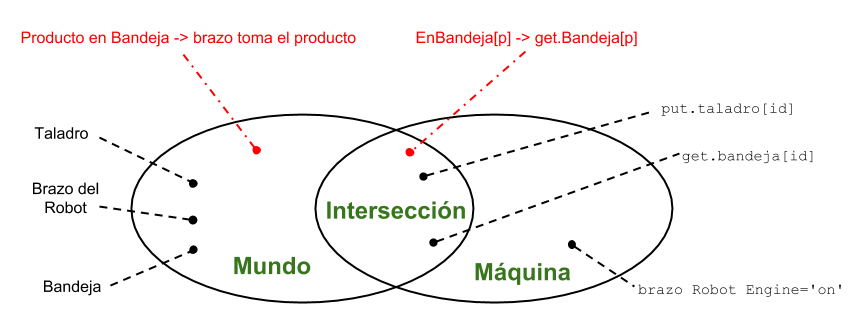
\includegraphics[scale=0.45]{img/world_and_machine.png}
    \caption{El Mundo y la Máquina}
    \label{world_and_machine}
\end{figure}

Así mismo, es esperado que la máquina proponga una solución al problema. Por ejemplo, en la Figura \ref{world_and_machine}
podemos ver que la célula de producción debe procesar cada producto, sólo si están disponible en la bandeja de entrada en ese
momento. Con la sentencia $EnBandeja[p] \rightarrow get.Bandeja[p]$ mostramos que se espera que el brazo del robot sólo
podrá tomar los productos de la bandeja cuando estén listos. Finalizando, los fenómenos compartidos entre el mundo y
máquina, es decir, los que se encuentran en la intersección, representa a la \emph{interfaz}, donde la máquina
interactúa con el mundo. También, podemos definir a los fenómenos del mundo como el \emph{modelo del entorno} ya que el
conjunto de éstos describen los eventos que suceden en el mundo real.

Las sentencias que detallan los distintos fenómenos, tanto en el mundo como en la máquina pueden variar en
\emph{alcance} y en \emph{forma} \cite{Parnas95functionaldocuments,Jackson:1995:SRA:210207}. Además, éstas pueden estar en modo \emph{indicativo} u \emph{optativo}. En
otros trabajos, como en \cite{van2009requirements}, las sentencias utilizadas son \emph{descriptivas} y \emph{prescriptivas}.

\begin{itemize}
    \item \underline{Sentencias descriptivas:} representan propiedades que son independientes de cómo se comporta el
    sistema. Se usan en modo \emph{indicativo}. No pueden ser cambiadas ni removidas.
    \item \underline{Sentencia prescriptivas:} afirman propiedades deseables que pueden estar presentes o no. Deben estar
    aplicadas por los componentes del sistema. Normalmente, pueden cambiar fortaleciéndose o debilitándose, o incluso
    pueden ser eliminadas. 
\end{itemize}

Anteriormente, fue mencionado que los estados pueden variar en su alcance. Ambos tipos de sentencias pueden referirse a
características de la máquina que no son compartidas por el mundo. En otras ocaciones, sentencias pueden referirse a
fenómenos compartidos por el mundo y la máquina. Más precisamente, una \emph{propiedad de dominio} es
una sentencia descriptiva sobre el mundo. Durante todo este trabajo, vamos a llamar \emph{modelo ambiente}, al conjunto
de propiedades del dominio de un problema particular.

Por otro lado, un \emph{supuesto de ambiente} es una sentencia que podría no suceder y debe ser satisfecha por el
ambiente. Un requisito de software, o \emph{requisito} de forma abreviada, es una sentencia prescriptiva que la máquina
deberá satisfacer independientemente de cómo se comporta el problema detallado en el mundo y deben ser elaboradas en
términos de fenómenos compartidos entre el mundo y la máquina.

Para finalizar y siguiendo lo publicado en \cite{VanLamsweerde:2001:GRE:882477.883624, 879820} podremos determinar a una
acción como supervisada/controlable si dicha acción es supervisada/controlable por la máquina. En este trabajo,
llamaremos a las acciones supervisadas como acciones no controlables, ya que están controladas por el ambiente.
